\chapter{Data}

We use a corpus of Bach chorales provided by \texttt{music21}. The chorales are
arranged by the Bach-Werke-Verzeichnis (BWV) numbering system, which is one of
the best known and widely used catalogues of Bach's compositions.

Each chorale has four parts and are structured such that the melody is in
the Soprano part and the remaining parts harmonize the melody.

\section{Preprocessing}

\begin{figure}[htpb]
    \centering
    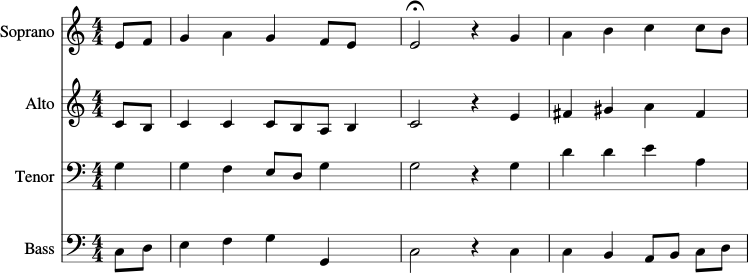
\includegraphics[width=1.0\linewidth]{Figures/bwv133-6-preproc-score-1.png}
    \caption{Score of BWV 133.6 after standardizing key and quantizing
    notes (see \autoref{fig:score-original} for original)}
    \label{fig:score-preproc}
\end{figure}

\begin{figure}[htpb]
    \centering
    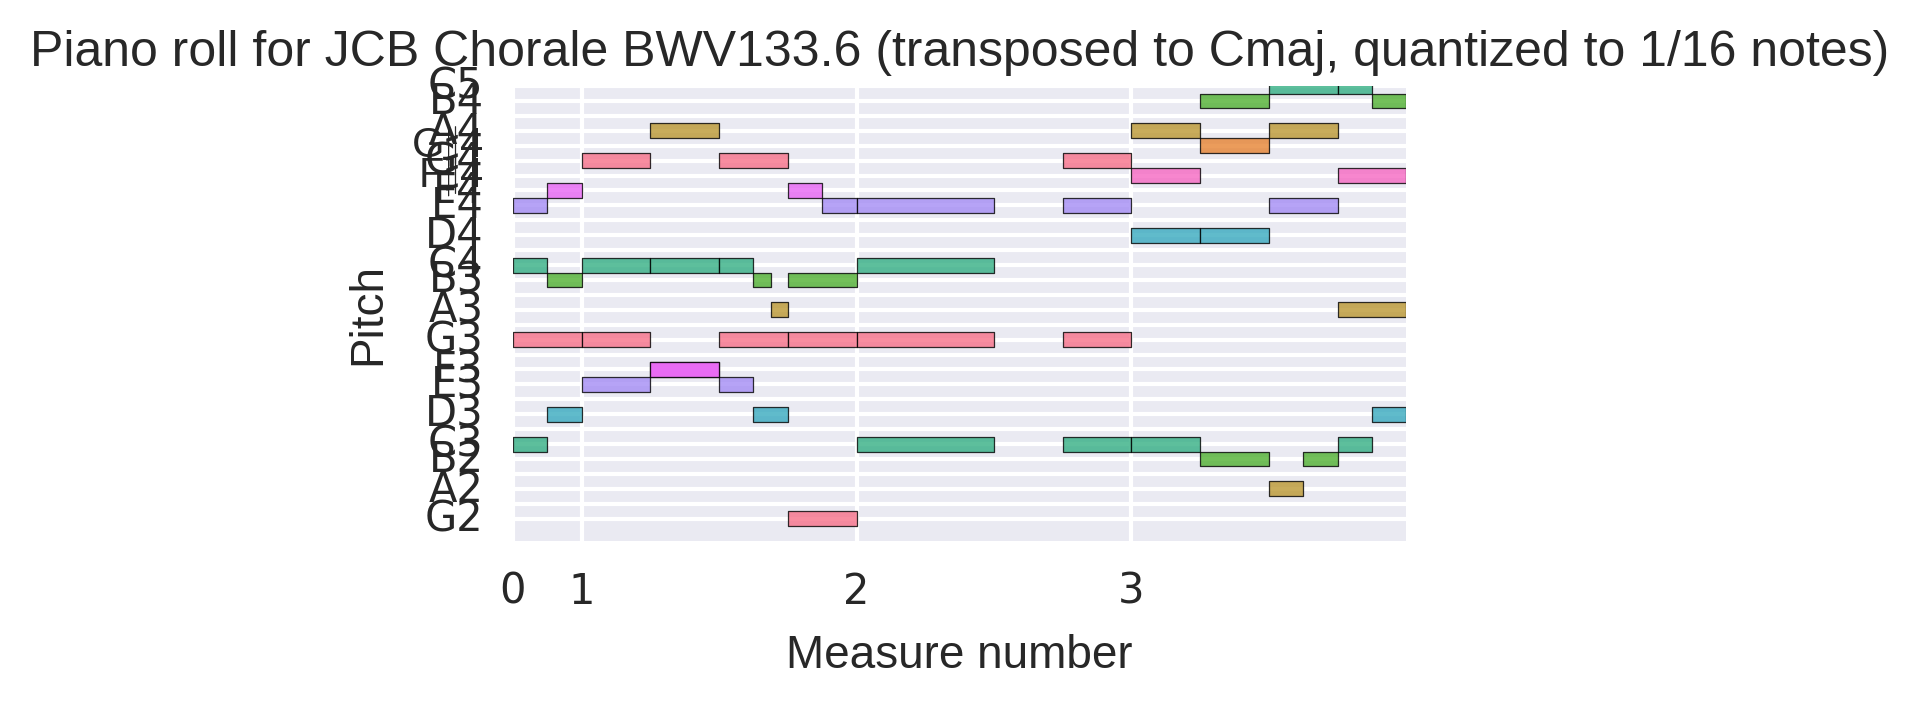
\includegraphics[width=1.0\linewidth]{Figures/bwv133-6-preproc-piano-roll.png}
    \caption{Piano roll of BWV 133.6 after standardizing key and quantizing
    notes (see \autoref{fig:piano-roll-original} for original)}
    \label{fig:piano-roll-preproc}
\end{figure}

We transpose all scores with major key signatures to C major and minor key
signatures to A minor. Due to transposition invariance of 12-TET, this does
not alter the tonal properties of the music.

We represent musical scores using a piano roll representation. Firstly, time is
discretized into constant timestep frames. For each frame, a set of (note, tie)
pairs representing which a note's pitch and whether it is tied
(continuing a note from the previous frame) or newly played notes.

\begin{enumerate}
    \item Transpose to Cmaj/Amin
    \item Strip all dynamics info
    \item Restrict to 4/4
\end{enumerate}

Both frame-based processing and quantization to eighth notes justified by Eck
and Smidhuber LSTM Blues \todo{cite}. Eight network time steps are required to
process a whole note. This is preferrable for the LSTM because it forces the network to learn
relative duration of notes, making it easier for counting and timing mechanisms
to be encoded by the LSTM dynamics \todo{Cite Gers and Schmidhuber, 2000}.

\textbf{Contribution}: solved problem of determining when notes end (\todo{cite
Eck Schmidhuber LSTM blues}) in input data format by using the ties.


